\begin{center}
    %%%%%%%%%%%%%%%%%%%%%%%%%%%%%%%%%
    %%%%%%%%%%%% Zoey's %%%%%%%%%%%%
    %%%%%%%%%%%%%%%%%%%%%%%%%%%%%%%%%
    \begin{tcolorbox}[colback=white, colframe=black, width=\textwidth, arc=6pt, boxrule=1pt]
        \sectiontitle{Pebble Motion Fidelity in PBRs}
        \sectioncontent{
            In pebble-bed reactors, the fuel movement varies greatly across the bed, pebble make multiple passess through the core,
            and different histroies have different burnup conditions. The heighest fidelity requires physics driven simulation\cite{richter}.

            \vspace{1em}

            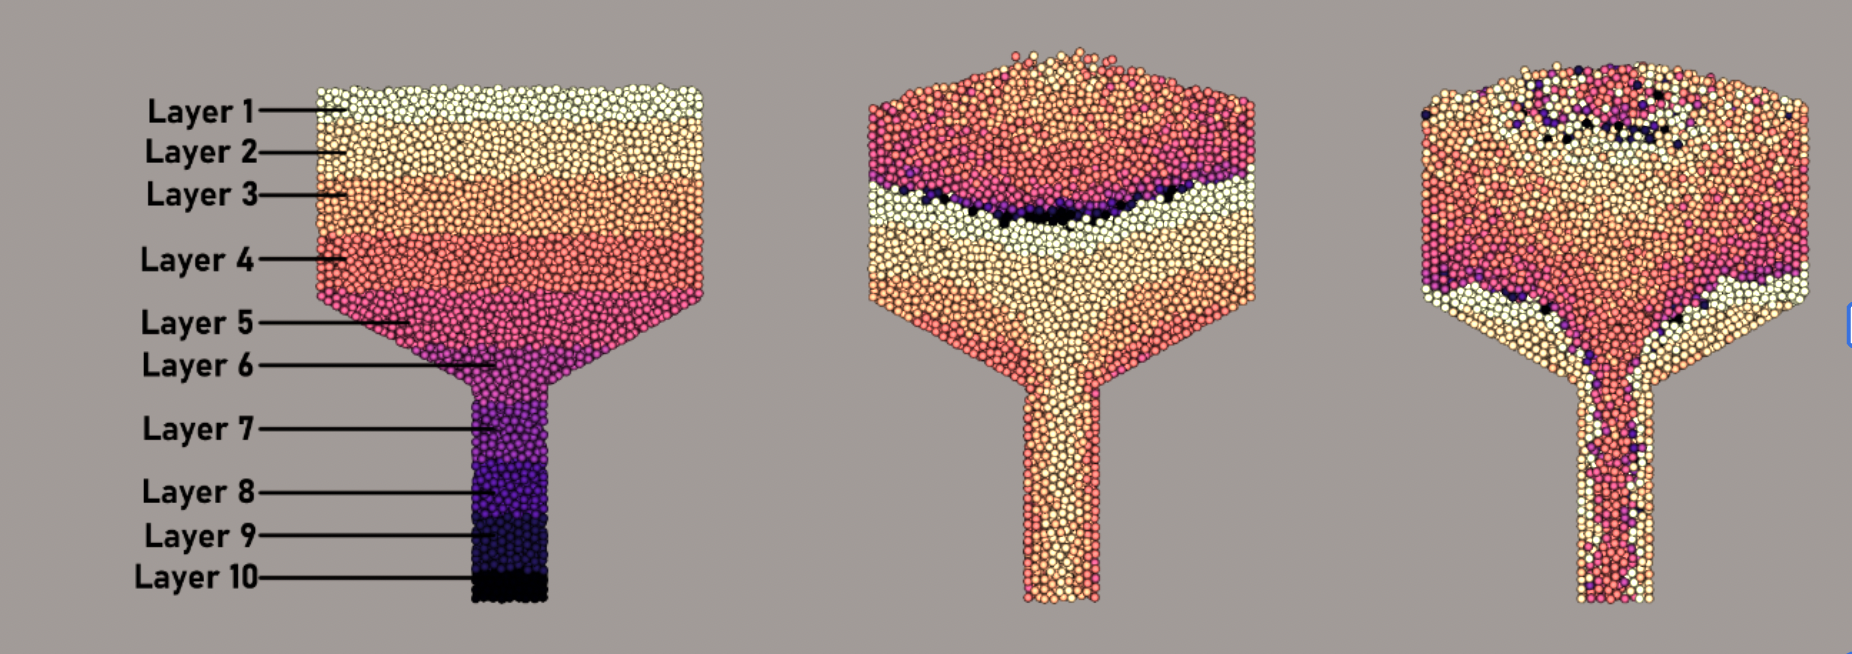
\includegraphics[width = 0.9\textwidth]{img/zoey1.png}

            \figcaption{Simulation of pebble circulation in different layers captured at zero days, 13 days, and 26 days.}

            \vspace{2em}

            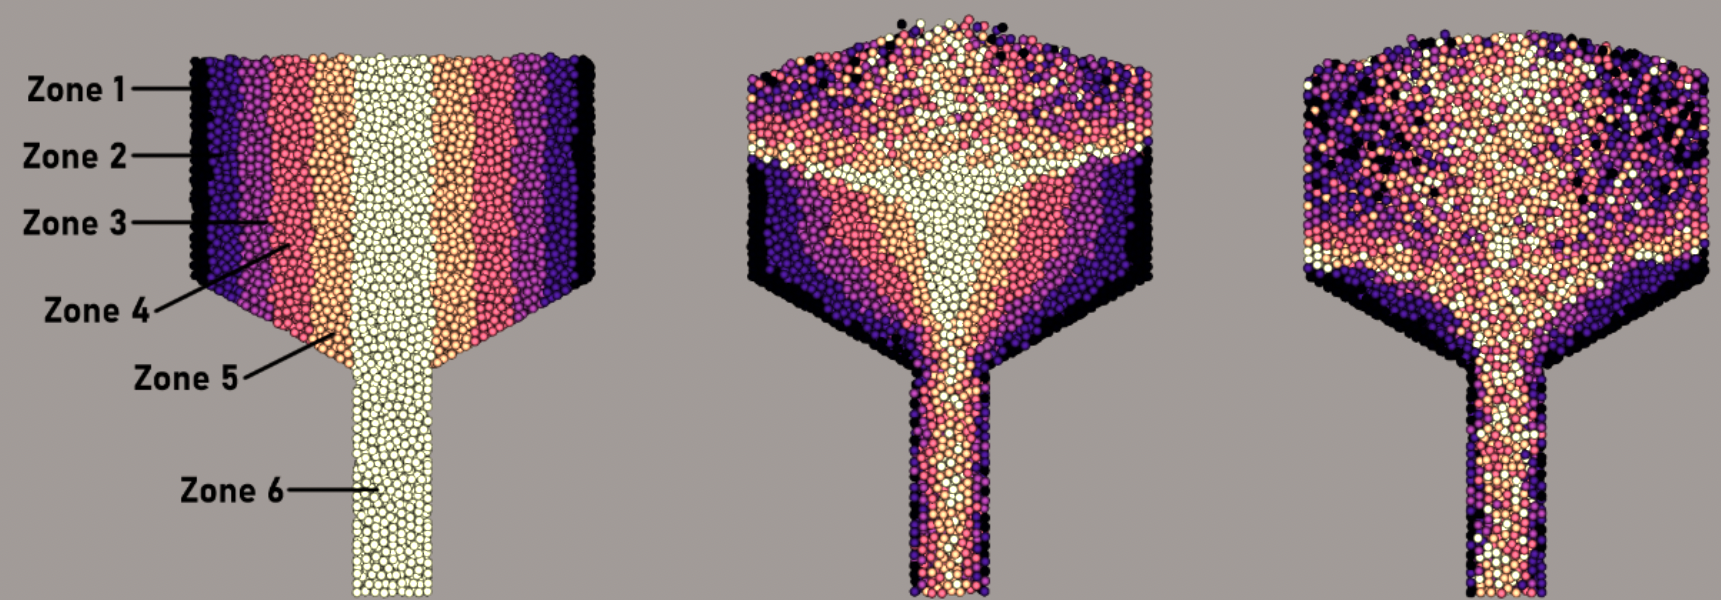
\includegraphics[width = 0.9\textwidth]{img/Zoey.png}

            \figcaption{Simulation of pebble movement in different zones captured at zero days, 13 days, and 26 days.}

            \begin{minipage}{.3\textwidth}
                \vspace{1em}
                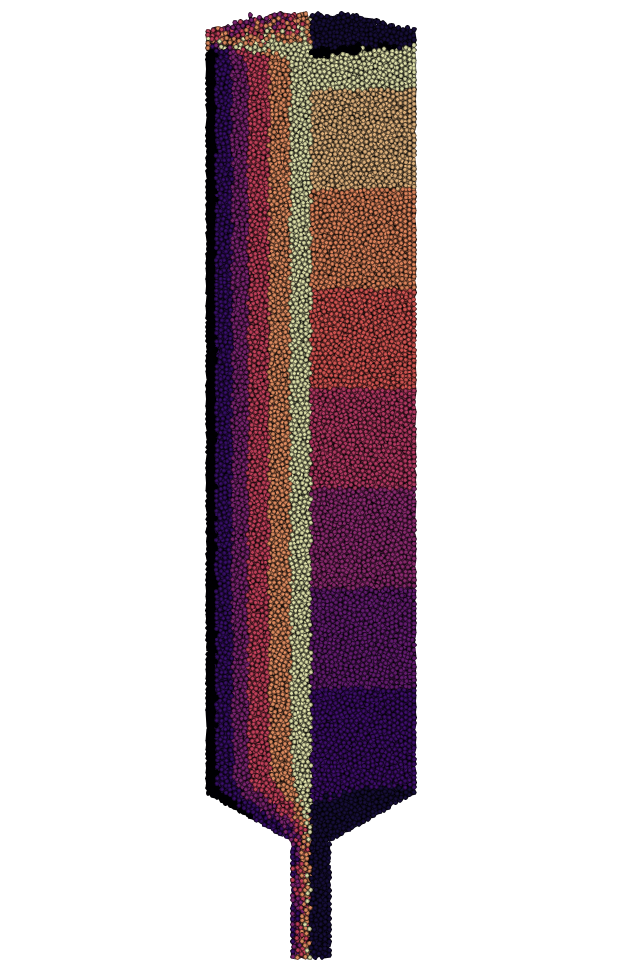
\includegraphics[width = \textwidth]{img/zonelayer.1682.png}
                \newline
                \figcaption{
                    Colors correspond to tracer labels.
                }
            \end{minipage}
            \hspace{0.5cm}
            \begin{minipage}{.3\textwidth}
                \vspace{1em}
                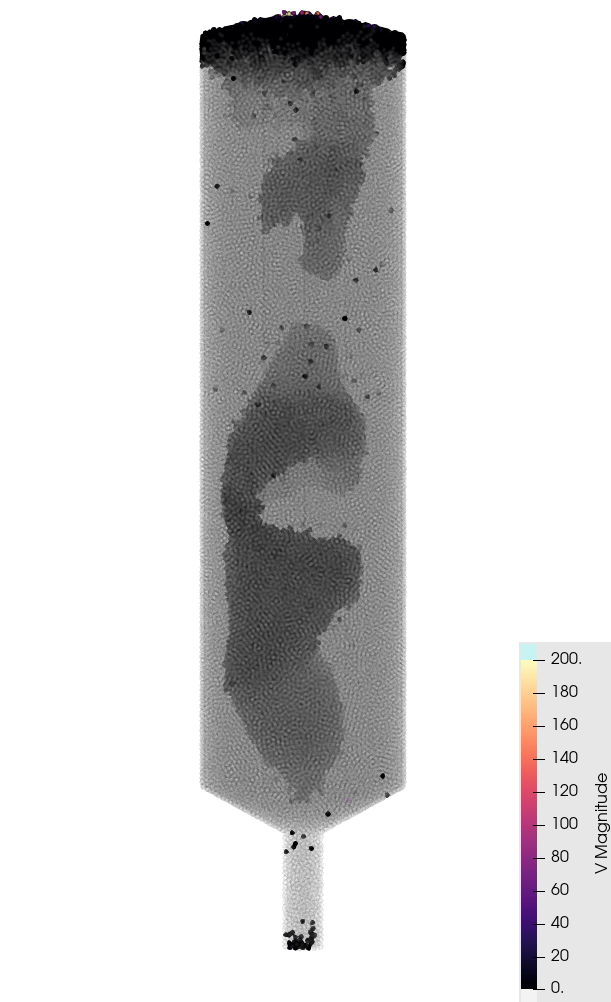
\includegraphics[width = \textwidth]{img/zoey2.png}
                \newline
                \figcaption{
                    Velocity magnitude [cm/s] of each pebble.
                }
            \end{minipage}
            \hspace{0.5cm}
            \begin{minipage}{.3\textwidth}
                \vspace{1em}
                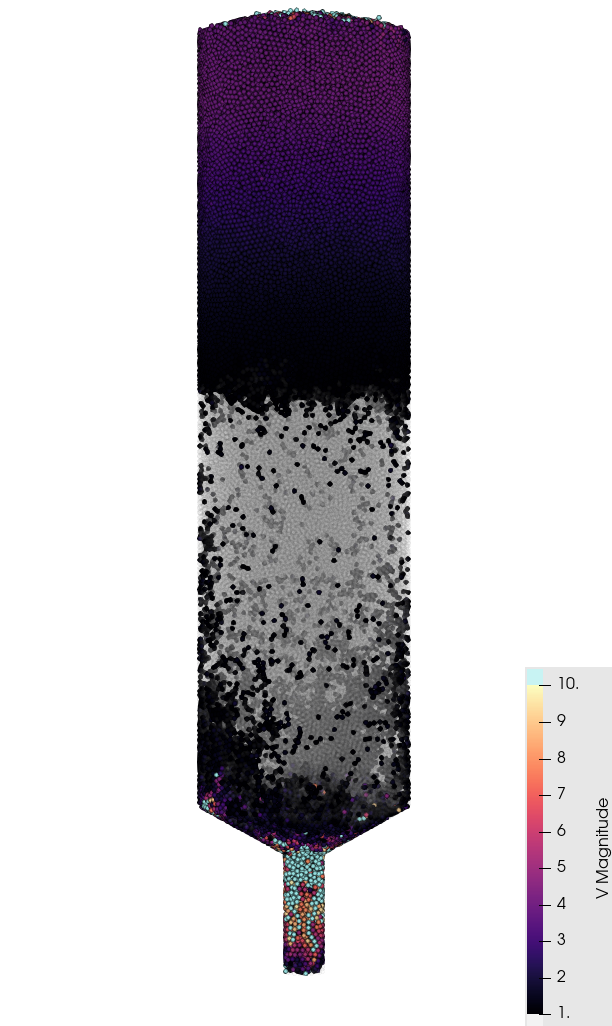
\includegraphics[width = \textwidth]{img/zoey3.png}
                \newline
                \figcaption{
                    Velocity magnitude [cm/s] of each pebble, with color map focused on slow pebbles.
                }
            \end{minipage}

        }
    \end{tcolorbox}

    %%%%%%%%%%%%%%%%%%%%%%%%%%%%%%%%
    %%%%%%%%% Luke's %%%%%%%%%%
    %%%%%%%%%%%%%%%%%%%%%%%%%%%%%%%%
    \begin{tcolorbox}[colback=white, colframe=black, width=\textwidth, arc=6pt, boxrule=1pt]
        \sectiontitle{Delayed Neutron Precursor Modeling}
        \sectioncontent{
	    Delayed neutron precursor experimental data is continuously being improved such that existing six group structures can be replicated computationally.
	    This approach can be leveraged to capture the effects of nuclear data uncertainties and advanced reactor phenomena. 

            \begin{minipage}{.45\textwidth}
                \vspace{1em}
                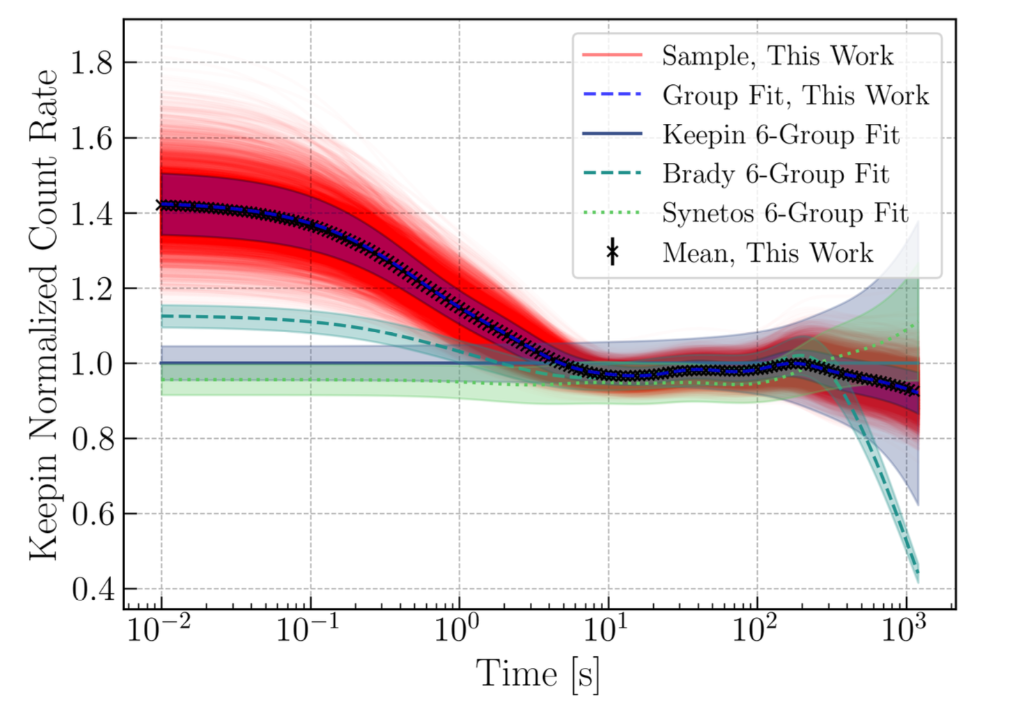
\includegraphics[width = 1\linewidth]{img/luke1.png}
		    \figcaption{The delayed neutron count rate for thermal fission of $^{235}$U normalized to the Keepin et al. six-group DNP group parameters \cite{keepin_delayed_1957}. The current work, represented by the Sampled, Group Fit, and Mean data trends shows poor agreement at times less than one second and agreement within uncertainty bounds beyond three seconds. These data are calculated using the IAEA $\beta$-delayed neutron emission database alongside ENDF/B-VII.1 cumulative fission yields \cite{dimitriou_development_2021, chadwick_endf_2011}.}
            \end{minipage}
            \hspace{1cm}
            \begin{minipage}{.45\textwidth}
                \vspace{1em}
		    \begin{center}
		    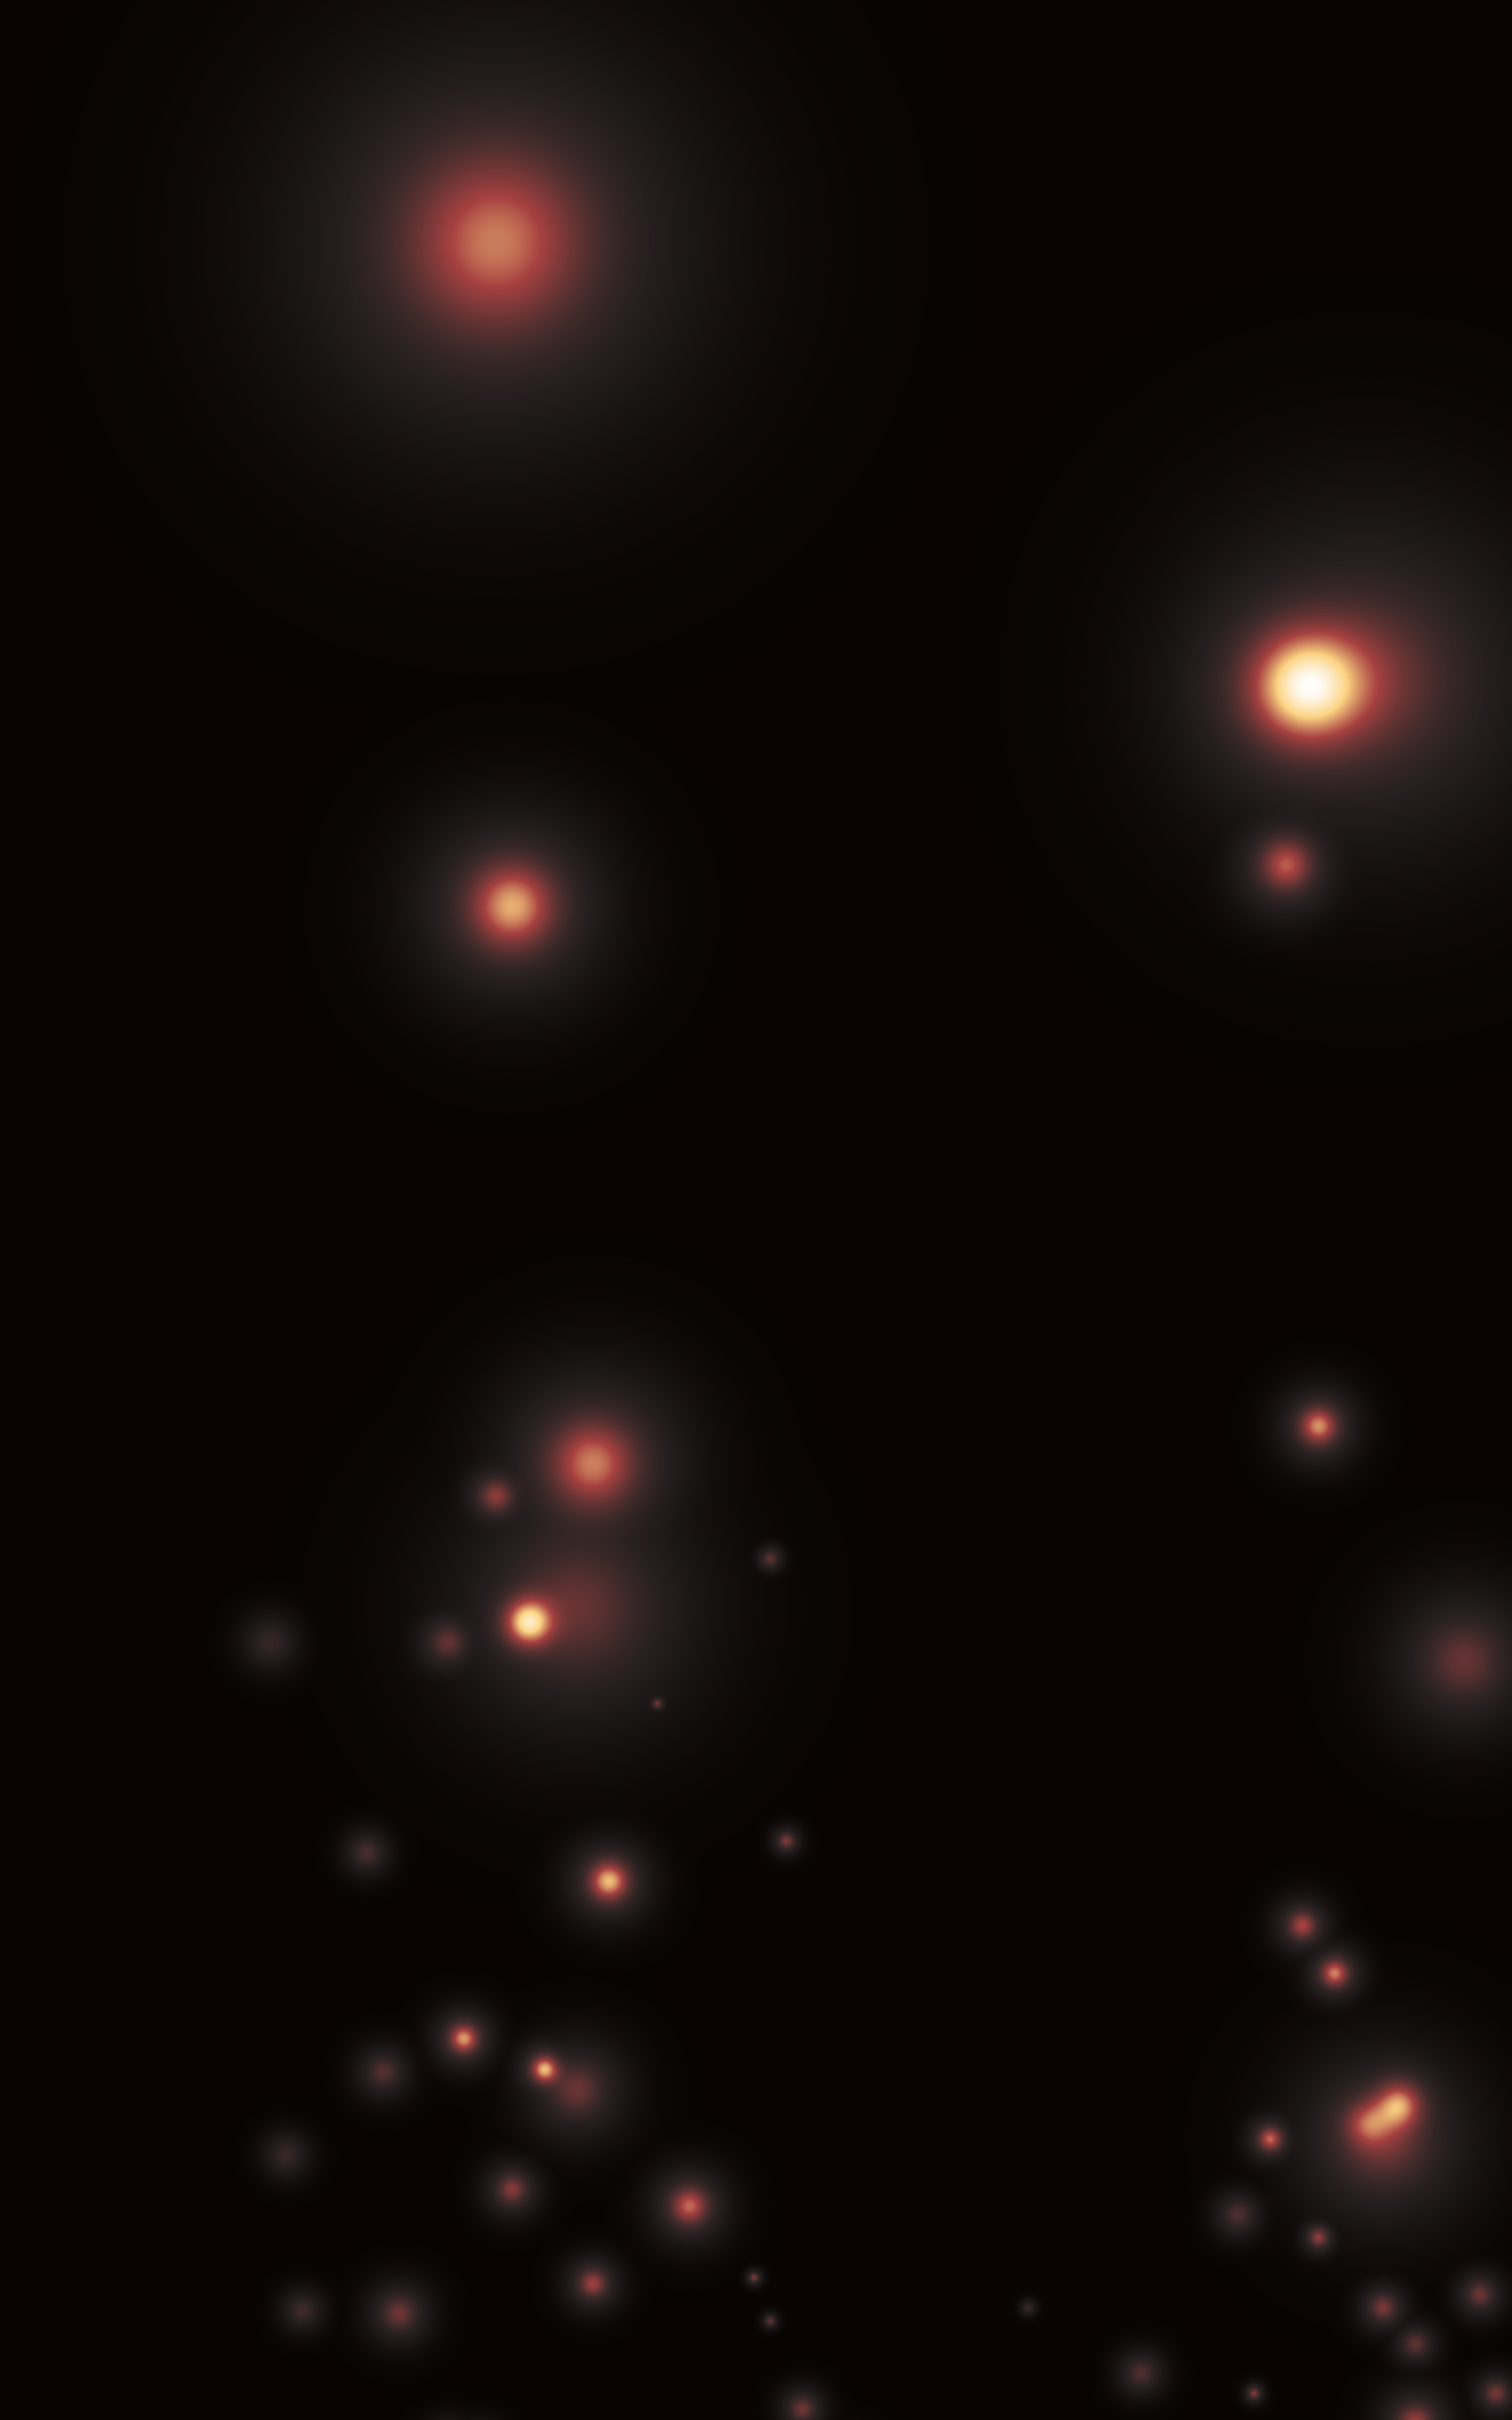
\includegraphics[height=12cm, width = 0.9\linewidth]{img/luke_seifert_1.png}
		    \end{center}
		    \figcaption{This is a qualitative visualization of the delayed neutron yields represented as embers from a fire. The yield data is plotted over atomic mass and the natural log of the half-life using the IAEA $\beta$-delayed neutron emission data and ENDF/B-VII.1 cumulative fission yields \cite{dimitriou_development_2021, chadwick_endf_2011}. The brightness of each ember indicates its delayed neutron yield during thermal fission of $^{235}$U, while the radius represents its uncertainty.}
            \end{minipage}
        }
    \end{tcolorbox}

    %%%%%%%%%%%%%%%%%%%%%%%%%%%%%%%%%
    %%%%%%%%%%%%% OLEK'S + Eli's%%%%%%%%%%%%%
    %%%%%%%%%%%%%%%%%%%%%%%%%%%%%%%%%
    \begin{tcolorbox}[colback=white, colframe=black, width=\textwidth, arc=6pt, boxrule=1pt]
        \sectiontitle{Transport Methods}
        \sectioncontent{
            content goes here
        }
    \end{tcolorbox}

    %%%%%%%%%%%%%%%%%%%%%%%%%%%%%%%%%

\end{center}
